\documentclass[10pt]{article}
\usepackage[polish]{babel}
\usepackage[utf8]{inputenc}
\usepackage[T1]{fontenc}
\usepackage{graphicx}
\usepackage[export]{adjustbox}
\graphicspath{ {./images/} }
\usepackage{amsmath}
\usepackage{amsfonts}
\usepackage{amssymb}
\usepackage[version=4]{mhchem}
\usepackage{stmaryrd}
\usepackage{multirow}

\title{EGZAMIN MATURALNY Z MATEMATYKI POZIOM PODSTAWOWY }

\author{}
\date{}


\newcommand\Varangle{\mathop{{<\!\!\!\!\!\text{\small)}}\:}\nolimits}

\begin{document}
\maketitle
\begin{center}
\begin{tabular}{|c|}
\hline
Miejsce \\
na naklejkę \\
z kodem szkoly \\
\hline
\end{tabular}
\end{center}

\begin{center}
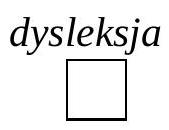
\includegraphics[max width=\textwidth]{2024_11_21_f98143b17bc89b1a1cceg-01}
\end{center}

MAJ ROK 2007

\section*{Czas pracy 120 minut}
\section*{Instrukcja dla zdającego}
\begin{enumerate}
  \item Sprawdź, czy arkusz egzaminacyjny zawiera 15 stron (zadania 1-11). Ewentualny brak zgłoś przewodniczącemu zespołu nadzorującego egzamin.
  \item Rozwiązania zadań i odpowiedzi zamieść w miejscu na to przeznaczonym.
  \item W rozwiązaniach zadań przedstaw tok rozumowania prowadzacy do ostatecznego wyniku.
  \item Pisz czytelnie. Używaj długopisu/pióra tylko z czarnym tuszem/atramentem.
  \item Nie używaj korektora, a błędne zapisy przekreśl.
  \item Pamiętaj, że zapisy w brudnopisie nie podlegają ocenie.
  \item Obok każdego zadania podana jest maksymalna liczba punktów, którą możesz uzyskać za jego poprawne rozwiązanie.
  \item Możesz korzystać z zestawu wzorów matematycznych, cyrkla i linijki oraz kalkulatora.
  \item Wypełnij tę część karty odpowiedzi, którą koduje zdajacy. Nie wpisuj żadnych znaków w części przeznaczonej dla egzaminatora.
  \item Na karcie odpowiedzi wpisz swoją datę urodzenia i PESEL. Zamaluj - pola odpowiadajace cyfrom numeru PESEL. Błędne zaznaczenie otocz kółkiem i zaznacz właściwe.\\

\includegraphics[max width=\textwidth, center]{2024_11_21_f98143b17bc89b1a1cceg-01(3)}
\end{enumerate}

Za rozwiązanie wszystkich zadań można otrzymać łacznie 50 punktów

Życzymy powodzenia!

Wypetnia zdający przed rozpoczęciem pracy\\
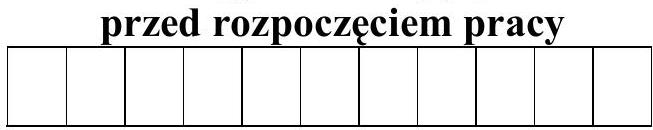
\includegraphics[max width=\textwidth, center]{2024_11_21_f98143b17bc89b1a1cceg-01(2)}

PESEL ZDAJĄCEGO\\
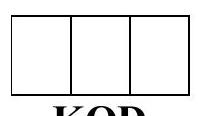
\includegraphics[max width=\textwidth, center]{2024_11_21_f98143b17bc89b1a1cceg-01(1)}

KOD\\
ZDAJĄCEGO

\section*{Zadanie 1. (5 pkt)}
Znajdź wzór funkcji kwadratowej \(y=f(x)\), której wykresem jest parabola o wierzchołku \((1,-9)\) przechodząca przez punkt o współrzędnych \((2,-8)\). Otrzymaną funkcję przedstaw w postaci kanonicznej. Oblicz jej miejsca zerowe i naszkicuj wykres.\\

\includegraphics[max width=\textwidth, center]{2024_11_21_f98143b17bc89b1a1cceg-02}

\begin{center}
\begin{tabular}{|c|l|c|c|c|c|c|}
\hline
\multirow{2}{*}{\begin{tabular}{c}
Wypetnia \\
egzaminator! \\
\end{tabular}} & Nr czynności & 1.1. & 1.2. & 1.3. & 1.4. & 1.5. \\
\cline { 2 - 7 }
 & Maks. liczba pkt & 1 & 1 & 1 & 1 & 1 \\
\cline { 2 - 7 }
 & Uzyskana liczba pkt &  &  &  &  &  \\
\hline
\end{tabular}
\end{center}

\section*{Zadanie 2. (3 pkt)}
Wysokość prowizji, którą klient płaci w pewnym biurze maklerskim przy każdej zawieranej transakcji kupna lub sprzedaży akcji jest uzależniona od wartości transakcji. Zależność ta została przedstawiona w tabeli:

\begin{center}
\begin{tabular}{|l|l|}
\hline
\multicolumn{1}{|c|}{Wartość transakcji} & \multicolumn{1}{c|}{Wysokość prowizji} \\
\hline
do \(500 \mathrm{zł}\) & \(15 \mathrm{zł}\) \\
\hline
od \(500,01 \mathrm{zł}\) do \(3000 \mathrm{zł}\) & \(2 \%\) wartości transakcji \(+5 \mathrm{zł}\) \\
\hline
od \(3000,01 \mathrm{zł}\) do \(8000 \mathrm{zł}\) & \(1,5 \%\) wartości transakcji \(+20 \mathrm{zł}\) \\
\hline
od \(8000,01 \mathrm{zł}\) do \(15000 \mathrm{zł}\) & \(1 \%\) wartości transakcji \(+60 \mathrm{zł}\) \\
\hline
powyżej \(15000 \mathrm{zł}\) & \(0,7 \%\) wartości transakcji \(+105 \mathrm{zł}\) \\
\hline
\end{tabular}
\end{center}

Klient zakupił za pośrednictwem tego biura maklerskiego 530 akcji w cenie \(25 \mathrm{zł}\) za jedna akcje. Po roku sprzedał wszystkie kupione akcje po 45 zł za jedną sztukę. Oblicz, ile zarobił na tych transakcjach po uwzględnieniu prowizji, które zapłacił.\\

\includegraphics[max width=\textwidth, center]{2024_11_21_f98143b17bc89b1a1cceg-03}

\begin{center}
\begin{tabular}{|c|l|c|c|c|}
\hline
\multirow{2}{*}{\begin{tabular}{c}
Wypelnia \\
egzaminator! \\
\end{tabular}} & Nr czynności & 2.1. & 2.2. & 2.3. \\
\cline { 2 - 5 }
 & Maks. liczba pkt & 1 & 1 & 1 \\
\cline { 2 - 5 }
 & Uzyskana liczba pkt &  &  &  \\
\hline
\end{tabular}
\end{center}

\section*{Zadanie 3. (4 pkt)}
Korzystając z danych przedstawionych na rysunku, oblicz wartość wyrażenia:\\
\(\operatorname{tg}^{2} \beta-5 \sin \beta \cdot \operatorname{ctg} \alpha+\sqrt{1-\cos ^{2} \alpha}\).\\
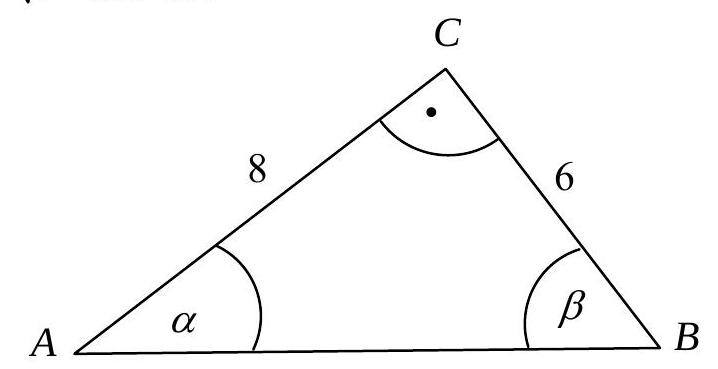
\includegraphics[max width=\textwidth, center]{2024_11_21_f98143b17bc89b1a1cceg-04}\\

\includegraphics[max width=\textwidth, center]{2024_11_21_f98143b17bc89b1a1cceg-04(1)}

\begin{center}
\begin{tabular}{|c|l|c|c|c|c|}
\hline
\multirow{2}{*}{\begin{tabular}{c}
Wypełnia \\
egzaminator! \\
\end{tabular}} & Nr czynności & 3.1. & 3.2. & 3.3. & 3.4. \\
\cline { 2 - 6 }
 & Maks. liczba pkt & 1 & 1 & 1 & 1 \\
\cline { 2 - 6 }
 & Uzyskana liczba pkt &  &  &  &  \\
\hline
\end{tabular}
\end{center}

\section*{Zadanie 4. (5 pkt)}
Samochód przebył w pewnym czasie 210 km . Gdyby jechał ze średnią prędkością o \(10 \mathrm{~km} / \mathrm{h}\) większa, to czas przejazdu skróciłby się o pół godziny. Oblicz, z jaką średnią prędkością jechał ten samochód.\\

\includegraphics[max width=\textwidth, center]{2024_11_21_f98143b17bc89b1a1cceg-05}

\begin{center}
\begin{tabular}{|c|l|c|c|c|c|c|}
\hline
\multirow{2}{*}{\begin{tabular}{c}
Wypelnia \\
egzaminator! \\
\end{tabular}} & Nr czynności & 4.1. & 4.2. & 4.3. & 4.4. & 4.5. \\
\cline { 2 - 7 }
 & Maks. liczba pkt & 1 & 1 & 1 & 1 & 1 \\
\cline { 2 - 7 }
 & Uzyskana liczba pkt &  &  &  &  &  \\
\hline
\end{tabular}
\end{center}

\section*{Zadanie 5. (5 pkt)}
Dany jest ciagg arytmetyczny \(\left(a_{n}\right)\), gdzie \(n \geq 1\). Wiadomo, że dla każdego \(n \geq 1\) suma \(n\) początkowych wyrazów \(S_{n}=a_{1}+a_{2}+\ldots+a_{n}\) wyraża się wzorem: \(S_{n}=-n^{2}+13 n\).\\
a) Wyznacz wzór na \(n\)-ty wyraz ciagu \(\left(a_{n}\right)\).\\
b) Oblicz \(a_{2007}\).\\
c) Wyznacz liczbę \(n\), dla której \(a_{n}=0\).\\

\includegraphics[max width=\textwidth, center]{2024_11_21_f98143b17bc89b1a1cceg-06}

\begin{center}
\begin{tabular}{|c|l|c|c|c|c|c|}
\hline
\multirow{2}{*}{\begin{tabular}{c}
Wypełnia \\
egzaminator! \\
\end{tabular}} & Nr czynności & 5.1. & 5.2. & 5.3. & 5.4. & 5.5. \\
\cline { 2 - 7 }
 & Maks. liczba pkt & 1 & 1 & 1 & 1 & 1 \\
\cline { 2 - 7 }
 & Uzyskana liczba pkt &  &  &  &  &  \\
\hline
\end{tabular}
\end{center}

\section*{Zadanie 6. (4 pkt)}
Dany jest wielomian \(W(x)=2 x^{3}+a x^{2}-14 x+b\).\\
a) Dla \(a=0\) i \(b=0\) otrzymamy wielomian \(W(x)=2 x^{3}-14 x\). Rozwiąż równanie \(2 x^{3}-14 x=0\).\\
b) Dobierz wartości \(a\) i \(b\) tak, aby wielomian \(W(x)\) był podzielny jednocześnie przez \(x-2\) oraz przez \(x+3\).\\

\includegraphics[max width=\textwidth, center]{2024_11_21_f98143b17bc89b1a1cceg-07}

\begin{center}
\begin{tabular}{|c|l|c|c|c|c|}
\hline
\multirow{2}{*}{\begin{tabular}{c}
Wypetnia \\
egzaminator! \\
\end{tabular}} & Nr czynności & 6.1. & 6.2. & 6.3. & 6.4. \\
\cline { 2 - 6 }
 & Maks. liczba pkt & 1 & 1 & 1 & 1 \\
\cline { 2 - 6 }
 & Uzyskana liczba pkt &  &  &  &  \\
\hline
\end{tabular}
\end{center}

\section*{Zadanie 7. (5 pkt)}
Dany jest punkt \(C=(2,3)\) i prosta o równaniu \(y=2 x-8\) będąca symetralną odcinka \(B C\).\\
Wyznacz współrzędne punktu \(B\). Wykonaj obliczenia uzasadniające odpowiedź.\\

\includegraphics[max width=\textwidth, center]{2024_11_21_f98143b17bc89b1a1cceg-08}

\section*{Zadanie 8. (4 pht)}
Na stole leżało 14 banknotów: 2 banknoty o nominale \(100 \mathrm{zz}, 2\) banknoty o nominale \(50 \mathrm{zł}\) i 10 banknotów o nominale \(20 \mathrm{zł}\). Wiatr zdmuchnął na podłogę 5 banknotów. Oblicz prawdopodobieństwo tego, że na podłodze leży dokładnie \(130 \mathrm{zł}\). Odpowiedź podaj w postaci ułamka nieskracalnego.\\

\includegraphics[max width=\textwidth, center]{2024_11_21_f98143b17bc89b1a1cceg-09}

\begin{center}
\begin{tabular}{|c|l|c|c|c|c|}
\hline
\multirow{2}{*}{\begin{tabular}{c}
Wypelnia \\
egzaminator! \\
\end{tabular}} & Nr czynności & 8.1. & 8.2. & 8.3. & 8.4. \\
\cline { 2 - 6 }
 & Maks. liczba pkt & 1 & 1 & 1 & 1 \\
\cline { 2 - 6 }
 & Uzyskana liczba pkt &  &  &  &  \\
\hline
\end{tabular}
\end{center}

\section*{Zadanie 9. (6 pkt)}
Oblicz pole czworokąta wypukłego \(A B C D\), w którym kąty wewnętrzne mają odpowiednio miary: \(\Varangle A=90^{\circ}, \Varangle B=75^{\circ}, \Varangle C=60^{\circ}, \Varangle D=135^{\circ}\), a boki \(A B\) i \(A D\) mają długość 3 cm . Sporządź rysunek pomocniczy.\\

\includegraphics[max width=\textwidth, center]{2024_11_21_f98143b17bc89b1a1cceg-10}\\

\includegraphics[max width=\textwidth, center]{2024_11_21_f98143b17bc89b1a1cceg-11}

\begin{center}
\begin{tabular}{|c|l|c|c|c|c|c|c|}
\hline
\multirow{2}{*}{\begin{tabular}{c}
Wypełnia \\
egzaminator! \\
\end{tabular}} & Nr czynności & 9.1. & 9.2. & 9.3. & 9.4. & 9.5. & 9.6. \\
\cline { 2 - 8 }
 & Maks. liczba pkt & 1 & 1 & 1 & 1 & 1 & 1 \\
\cline { 2 - 8 }
 & Uzyskana liczba pkt &  &  &  &  &  &  \\
\hline
\end{tabular}
\end{center}

\section*{Zadanie 10. (5 pkt)}
Dany jest graniastosłup czworokatny prosty ABCDEFGH o podstawach ABCD i EFGH oraz krawędziach bocznych \(A E, B F, C G, D H\). Podstawa \(A B C D\) graniastosłupa jest rombem o boku długości 8 cm i kątach ostrych \(A\) i \(C\) o mierze \(60^{\circ}\). Przekątna graniastosłupa \(C E\) jest nachylona do płaszczyzny podstawy pod kątem \(60^{\circ}\). Sporządź rysunek pomocniczy i zaznacz na nim wymienione w zadaniu kąty. Oblicz objętość tego graniastosłupa.\\

\includegraphics[max width=\textwidth, center]{2024_11_21_f98143b17bc89b1a1cceg-12}\\

\includegraphics[max width=\textwidth, center]{2024_11_21_f98143b17bc89b1a1cceg-13}

\begin{center}
\begin{tabular}{|c|c|c|c|c|c|c|}
\hline
\multirow{2}{*}{\begin{tabular}{c}
Wypełnia \\
egzaminator! \\
\end{tabular}} & Nr czynności & 10.1. & 10.2. & 10.3. & 10.4. & 10.5. \\
\cline { 2 - 7 }
 & Maks. liczba pkt & 1 & 1 & 1 & 1 & 1 \\
\hline
 & Uzyskana liczba pkt &  &  &  &  &  \\
\hline
\end{tabular}
\end{center}

\section*{Zadanie 11. (4 pkt)}
Dany jest rosnący ciag geometryczny \(\left(a_{n}\right)\) dla \(n \geq 1\), w którym \(a_{1}=x, a_{2}=14, a_{3}=y\). Oblicz \(x\) oraz \(y\), jeżeli wiadomo, że \(x+y=35\).\\

\includegraphics[max width=\textwidth, center]{2024_11_21_f98143b17bc89b1a1cceg-14}

\begin{center}
\begin{tabular}{|c|c|c|c|c|c|}
\hline
\multirow{2}{*}{\begin{tabular}{c}
Wypelnia \\
egzaminator! \\
\end{tabular}} & Nr czynności & 11.1. & 11.2. & 11.3. & 11.4. \\
\cline { 2 - 6 }
 & Maks. liczba pkt & 1 & 1 & 1 & 1 \\
\cline { 2 - 6 }
 & Uzyskana liczba pkt &  &  &  &  \\
\hline
\end{tabular}
\end{center}

\section*{BRUDNOPIS}

\end{document}